\chapter{Romberg quadrature}

\section{The algorithm}

Let \(f:[a,b] \rightarrow \R\) be a function and \(I\coloneqq \int_a^bf(x)dx\). The {\it trapezoidal rule} is a method for approaching \(I\) which works as follows: Let \(a = t_0 < t_1 < \cdots < t_n = b\) be a subdivision of \([a,b]\). On each of the intervals \([t_{i-1},t_i]\) we approximate \(\int_{t_{i-1}}^{t_i}f(x)dx\) by the area of a trapezoid with verticies \((t_{i-1},0),\,(t_{i-1}, f(t_{i-1})),\,(t_i,f(t_i)),\, (t_i,0)\) i.e. by \(\frac{1}{2}(t_i - t_{i-1})(f(t_{i-1}) + f(t_i))\). Hence we approximate \(I\) by 

\[
I = \sum_{i=1}^n \int_{t_{i-1}}^{t_i}f(x)dx \approx \sum_{i=1}^n\frac{1}{2}(t_i - t_{i-1})(f(t_{i-1}) + f(t_i)).
\]
If \(t_i - t_{i-1} = \frac{1}{n}(b-a)\eqqcolon h\) for each \(i\) then the above estimate becomes
\begin{equation}\label{trapezoidal}
I \approx h \left(\frac{1}{2}(f(a) + f(b)) + \sum_{i=1}^{n-1}f(a + ih)\right)
\end{equation}
We define \(T_f(h)\) as the right hand side in (\ref{trapezoidal}).\\

Let \(F:[0, n]\rightarrow \R\) be a \(2k+1\) times continuously differentiable function, \(n\) a positive integer. Then by Euler's summation formula (see formula 298 in \cite{kn}) we have
\begin{equation}
\sum_{i=0}^nF(i) = \int_0^nF(x)dx + \frac{1}{2}(F(0) + F(n)) + \sum_{i=1}^k\frac{B_{2i}}{(2i)!}(F^{(2i-1)}(n) - F^{(2i-1)}(0)) + R_k
\end{equation}
where \(R_k = \int_0^nP_{2k+1}(x)F^{(2k+1)}(x)dx\), \(B_m\) are the {\it Bernoulli numbers} and \(P_m\) the {\it Bernoulli polynomials.} If let \(F(x)\coloneqq f(a + xh)\) then we get the following asymptotic expansion for the trapezoidal rule:

\begin{theorem}
Let \(f:[a,b] \rightarrow \R\) be \(2k+1\) times continuously differentiable and \(h \coloneqq (b-a)/n\). Then 
\begin{equation}
T_f(h) = I + \sum_{i=1}^k\frac{B_{2i}}{(2i)!}(f^{(2i-1)}(b) - f^{(2i-1)}(a))h^{2i} + h^{2k+1}R_k(h)
\end{equation}
where
\begin{equation}
R_k(h) = \int_a^bP_{k+1}\left(n\frac{x-a}{b-a}\right)f^{(2k+1)}(x)dx. 
\end{equation}
\end{theorem}

The following code is a trivial implementation of the trapezoidal rule. The {\it TrapezoidalRule} class in an implementation of the abstract class {\it Scheme} which represents a numerical scheme or method, which has asymptotic expansion in \(h^p\). The Scheme class has a method named {\it apply} which takes in a problem to which the scheme is applied to. The argument \(m\) in the apply-method is the number of subintervals that should be used.

\begin{minted}[tabsize=2, fontsize=\footnotesize]{python}
class TrapezoidalRule(Scheme):
    def __init__(self):
        super(TrapezoidalRule, self).__init__(2)

    def apply(self, inte, m):
        (a,b) = inte.interval
        h = (b - a) / m
        I = 0.5 * (inte.f(a) + inte.f(b))
        for i in range(1, m):
            I += inte.f(a + i * h)

        return I * h
\end{minted}

Assume that we have computed the value of \(T_f(h)\) for \(h = h_1,\ldots,h_k\) and we want extrapolate to zero, i.e. we want to compute the value at zero of the interpolation polynomial in \(h^2\) for \((h_i^2,T_f(h_i)\), \(i=1,\ldots,k\). Denote by \(T_{ij}\) the value at zero of the polynomial in \(h^2\) which goes through \((h_{i-j+1}^2, T(h_{i-j+1}),\ldots,(h_i^2,T(h_i))\). The Neville scheme gives us the following algorithm for computing \(T_{ij}\), \(1\leq j\leq i\leq k\), recursively:

\begin{enumerate}
    \item \(T_{i1} \coloneqq T_f(h_i)\) for \(i = 1,\ldots,k\).
    \item \(T_{ij} \coloneqq T_{i,j-1} + \frac{T_{i,j-1} - T_{i-1,j-1}}{\left(\frac{h_{i-j+1}}{h_i}\right)^2 - 1}\) for \(2\leq j\leq i\).
\end{enumerate}

\section{Numerical experiments}

In this section we are going to apply Romberg quadrature to various functions and also try different sequences. We will analyze how different sequences perform in the sense that we want to measure how many function evaluations we need to attain a prescribed precision.\\

We will try various functions and the following sequences:
\begin{itemize}
    \item The harmonic sequence: \(a_n = n\), \(n\geq 0\).
    \item The Romberg sequence: \(a_n = 2^{n-1}\), \(n\geq 1\).
    \item The Bulirsch sequence: \(a_1 = 1\), \(a_2 = 2\), \(a_3 = 3\) and \(a_{n+2} = 2\cdot a_n\) for \(n\geq 2\). Its first elements are 
    \[
    1,\, 2,\, 3,\, 4,\, 6,\, 8,\, 12,\, 16,\, 24,\, 32,\ldots
    \]
\end{itemize}
Suppose that we are approximating the integral \(I\coloneqq \int_a^b f(x)dx\) using Romberg quadrature. We will use the stepsizes \(h_k\coloneqq (b-a)/a_k\) for the extrapolation. Let \(T_{ij}\), \(i\geq 0\) and \(j\leq i\) be the extrapolation table we get and \(\varepsilon_k \coloneqq |T_{kk}-I|\) be the error on the diagnoals. Let \(N_k\) be the number of function evaluations needed to compute \(T_{kk}\). We will use \(N_k\) as the measurement of computational effort as mentioned in section 1.3 and we will try to fit the exponential convergence model introduced there. We will also plot the logarithm of the error against the number of extrapolation steps. Note that \(N_k = \sum_{i=1}^k(a_i + 1)\) where \((a_i)\) is our sequence, so in case of the Harmonic sequence, we have \(N_n = n(n+3)/2 \approx n^2/2\) for \(n\) large. Hence if \(\varepsilon_n \sim A\exp(-cN_n^q)\) then 
\[
\varepsilon_n \sim A\exp(-c/2^qn^{2q})
\]
for \(n\) large. Thus if the error converges exponentially with the number of function evaluations, it will also converge exponentially with the number of extrapolation steps, and the exponent in the latter fitting will be twice the parameter from the former.\\

If our sequence is the Romberg sequence then \(N_k = \sum_{i=1}^n (2^{i-1} + 1) = 2^k + k - 1 \approx 2^k\) for \(k\) large, so if \(\varepsilon_k\sim A \exp(-cN_k^q)\) then 
\[
\varepsilon_k \sim A\exp(-c 2^{kq}) 
\]
for \(k\) large, which is not exponential convergence. On the other hand, if the we have exponential convergence in the number of extrapolation steps, i.e.
\[
\varepsilon_k \sim A \exp(-c k^q)
\]
then since \(k \approx \ln N_k / \ln 2\) we get 
\[
\ln \varepsilon_k \sim \ln A - c (\ln N_k / \ln 2)^q = \ln A - \frac{c}{(\ln 2)^q} (\ln N_k)^q
\]
so if we consider the ln-ln plot of the error against the number of function evaluations, then the points should fall on the graph of a function of the form \(t\mapsto b - c t^q\). The exponent should be the same as in the fitting for the logarithm of the error against the number of extrapolation steps.\\

For the model fitting we will thus plot the logarithm of the error agains the number of function evaluations, the number of extrapolation steps and the logarithm of the number of extrapolation steps. We will also consider the plot of the base \(10\) logarithm of the error against the number of function evaluations.\\

We conduct the experiments in Python 3 and use the high precision arithmetic library mpmath for all the computations. The precision will be set to \(500\) significant digits so will not have to worry about numerical instabilities.\\

Now we will consider the results of the experiments.

\subsection{Cosine squared}
The first function we are going to try is
\[
f: [0, \pi]\rightarrow \R, \quad f(x) \coloneqq \cos^2(x)
\]
which is entire.

%cos^2(x)
\begin{figure}[H]
\centering
\begin{minipage}{0.45\textwidth}
\centering
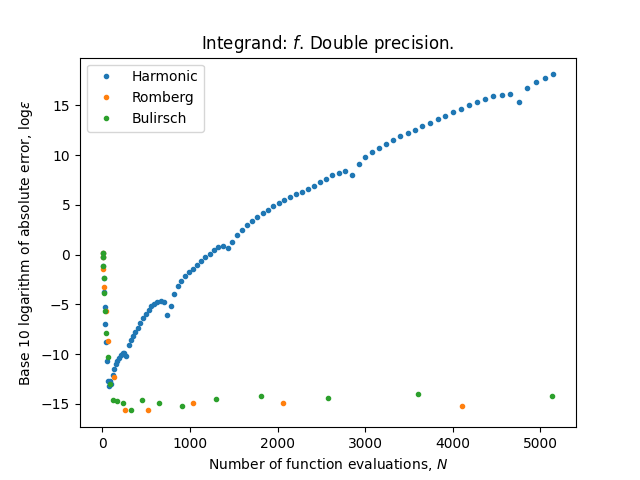
\includegraphics[scale=0.45]{romberg_plots/cos_squared.png}
\end{minipage}
\begin{minipage}{0.45\textwidth}
\centering
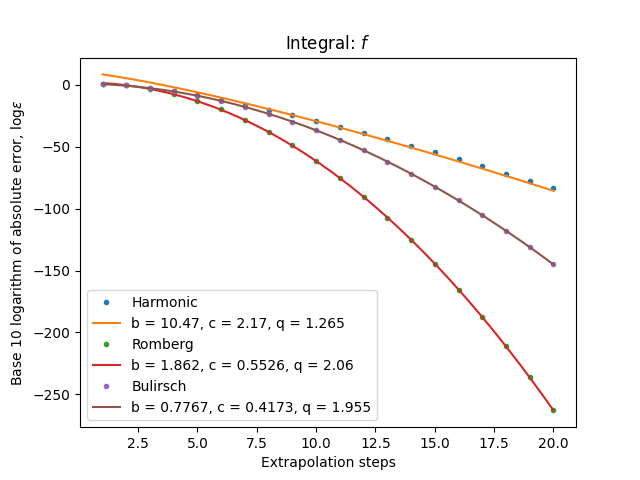
\includegraphics[scale=0.45]{romberg_plots/cos_squared_hp_steps.png}
\end{minipage}
\end{figure}

\begin{figure}[H]
\centering
\begin{minipage}{0.45\textwidth}
\centering
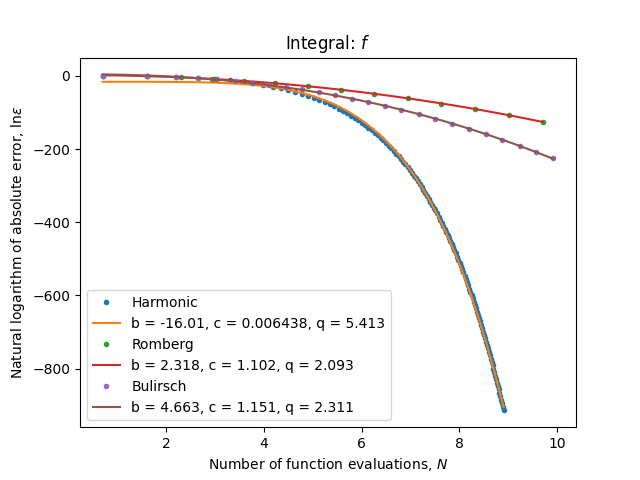
\includegraphics[scale=0.45]{romberg_plots/cos_squared_hp_log_log_pow_fit_trend.png}
\end{minipage}
\begin{minipage}{0.45\textwidth}
\centering
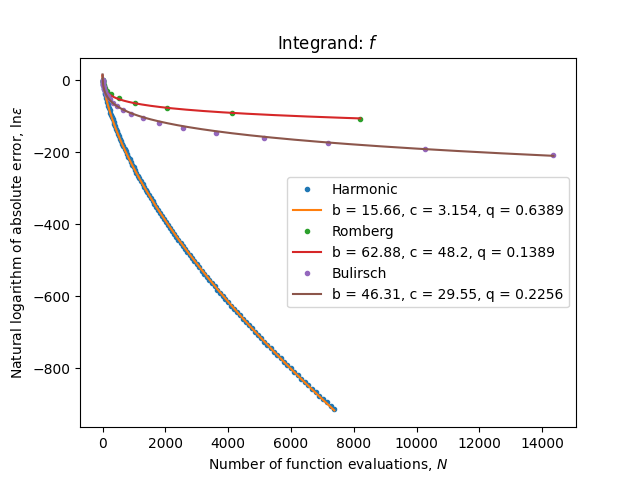
\includegraphics[scale=0.45]{romberg_plots/cos_squared_hp_trend.png}
\end{minipage}
\end{figure}

When considering the number of function evaluations against the error we seem to have exponential convergence for the Harmonic sequence. We reject the fitting for the fitting of the exponential convergence model, for Romberg and Bulirsch, since the \(b\) parameter is unreasonably large for an exponent. However, we seem to have exponential convergence in all cases when considering the number of extrapolation steps against the error.\\

The Harmonic sequence performes best, then Bulirsch and then Romberg. In standard double precision floating point arithmetic, we get down to maching level error using any sequence. Regarding convergence with the number of extrapolation, then it looks as we have exponential convergence for the Romberg and Bulirsch sequences.

\subsection{Function with poles}

Now we will consider the following function:
\[
g_a: [-1, 1] \rightarrow \R, \quad g_a(x) \coloneqq \frac{1}{a^2 + x^2},\, a > 0
\]
\begin{figure}[H]
\centering
\begin{minipage}{0.45\textwidth}
\centering
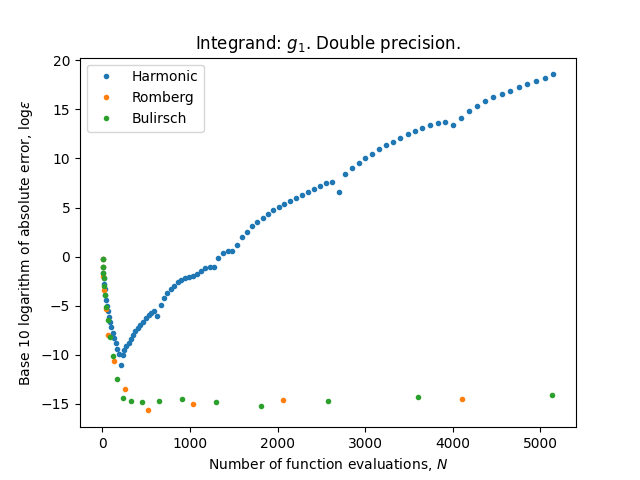
\includegraphics[scale=0.45]{romberg_plots/g_one.png}
\end{minipage}
\begin{minipage}{0.45\textwidth}
\centering
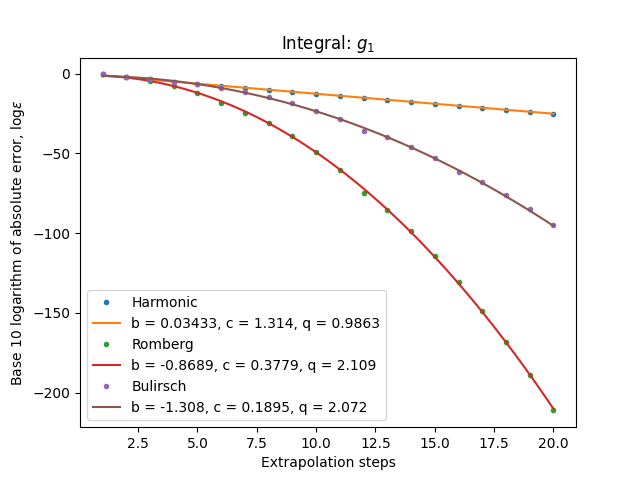
\includegraphics[scale=0.45]{romberg_plots/g_one_hp_steps.png}
\end{minipage}
\end{figure}

\begin{figure}[H]
\centering
\begin{minipage}{0.45\textwidth}
\centering
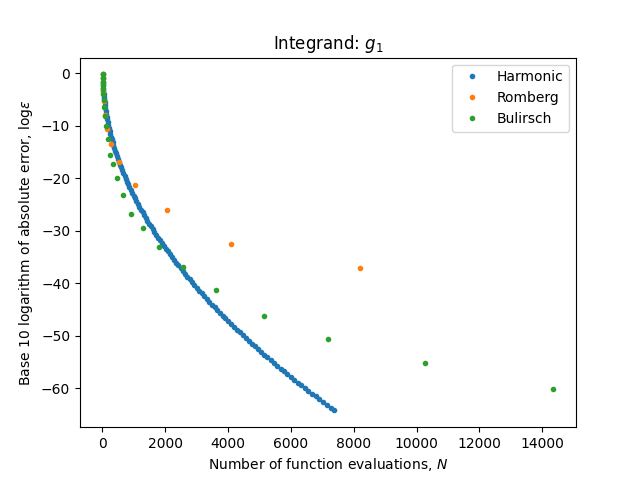
\includegraphics[scale=0.45]{romberg_plots/g_one_hp.png}
\end{minipage}
\begin{minipage}{0.45\textwidth}
\centering
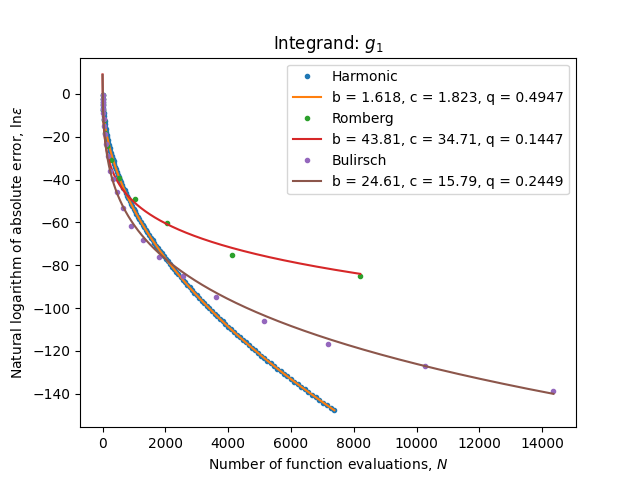
\includegraphics[scale=0.45]{romberg_plots/g_one_hp_trend.png}
\end{minipage}
\end{figure}

The error seems to converge exponentally with the number of function evaluations for the harmonic sequence but again the \(b\) parameters are unreasonably big for the other two sequences. For the number of extrapolation steps against the error, we seem to have exponential convergence in all cases. In standard floating point arithmetic, we get down to machine level precision for the Romberg and Bulirsch sequences but not for the Harmonic sequence. At first the sequences perform simarly but in the long run the harmonic sequence results in the fastest convergence.

\begin{figure}[H]
\centering
\begin{minipage}{0.45\textwidth}
\centering
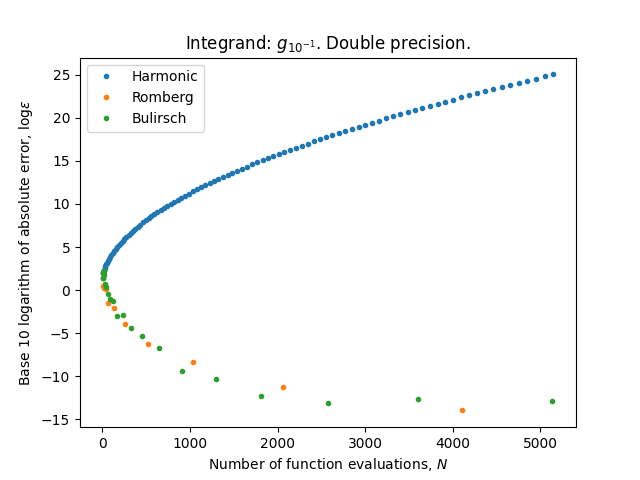
\includegraphics[scale=0.45]{romberg_plots/g_tenth.png}
\end{minipage}
\begin{minipage}{0.45\textwidth}
\centering
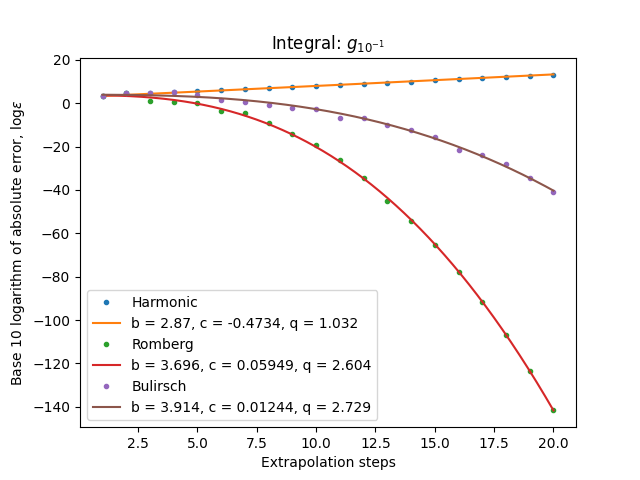
\includegraphics[scale=0.45]{romberg_plots/g_tenth_hp_steps.png}
\end{minipage}
\end{figure}

\begin{figure}[H]
\centering
\begin{minipage}{0.45\textwidth}
\centering
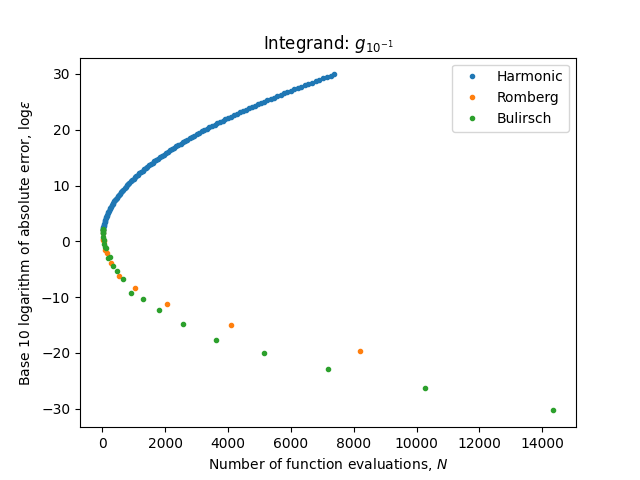
\includegraphics[scale=0.45]{romberg_plots/g_tenth_hp.png}
\end{minipage}
\begin{minipage}{0.45\textwidth}
\centering
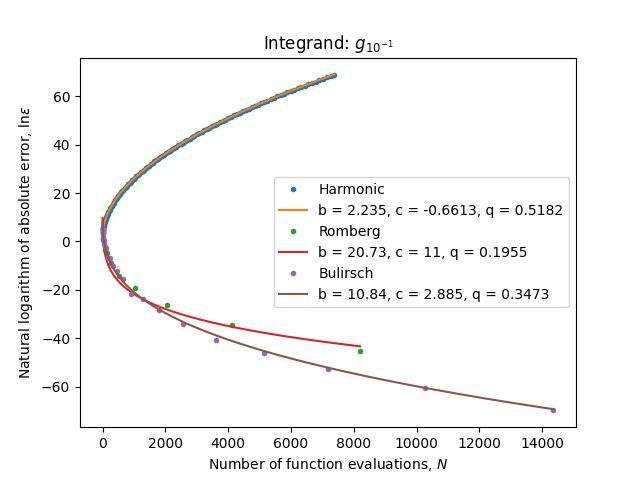
\includegraphics[scale=0.45]{romberg_plots/g_tenth_hp_trend.png}
\end{minipage}
\end{figure}

\begin{figure}[H]
\centering
\begin{minipage}{0.45\textwidth}
\centering
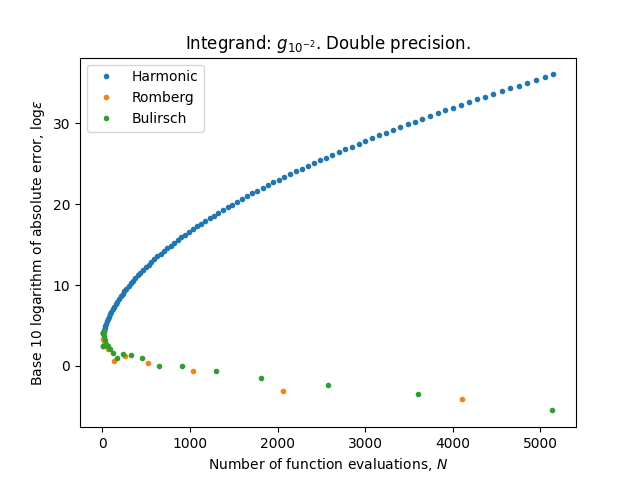
\includegraphics[scale=0.45]{romberg_plots/g_hundredth.png}
\end{minipage}
\begin{minipage}{0.45\textwidth}
\centering
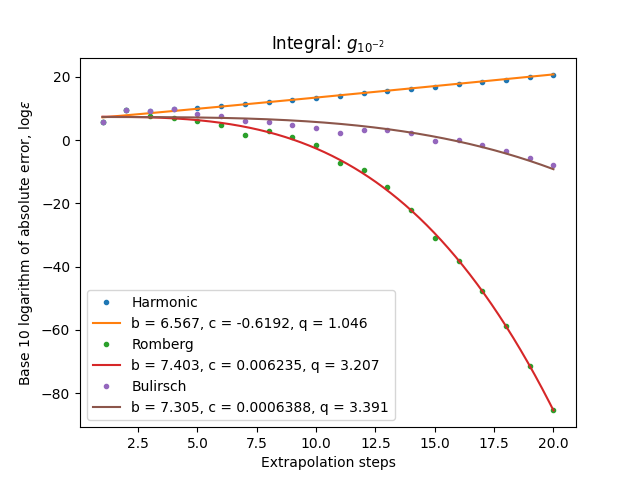
\includegraphics[scale=0.45]{romberg_plots/g_hundredth_hp_steps.png}
\end{minipage}
\end{figure}

\begin{figure}[H]
\centering
\begin{minipage}{0.45\textwidth}
\centering
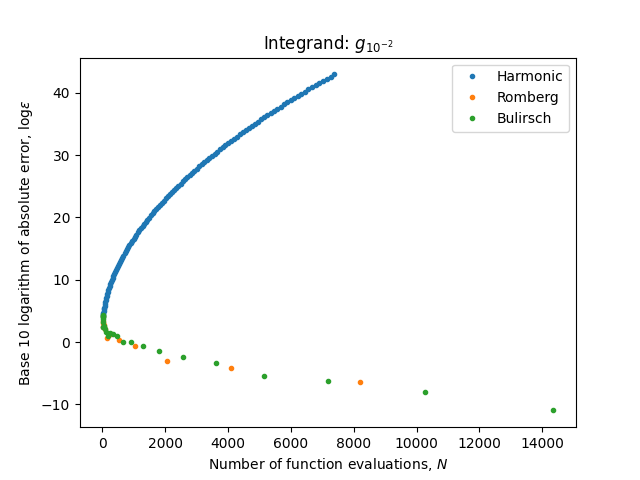
\includegraphics[scale=0.45]{romberg_plots/g_hundredth_hp.png}
\end{minipage}
\begin{minipage}{0.45\textwidth}
\centering
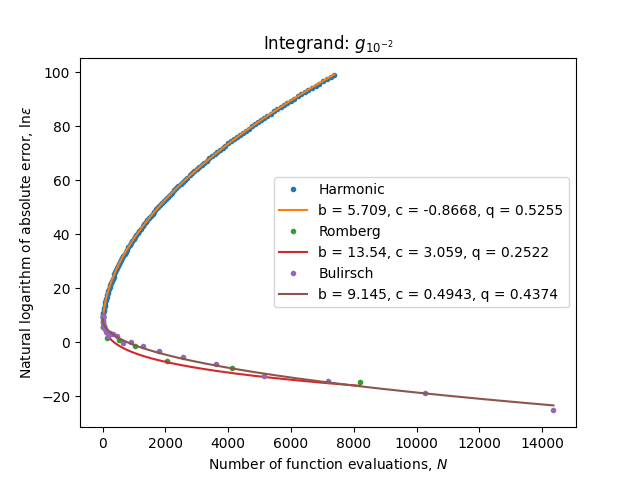
\includegraphics[scale=0.45]{romberg_plots/g_hundredth_hp_trend.png}
\end{minipage}
\end{figure}

For \(a = 10^{-1}, 10^{-2}\) we get divergence for the harmonic sequence, Bulirsch performes best for \(a = 10^{-1}\) and Romberg for \(a = 10^{-2}\). The parameters in the fitting of the exponential convergence model to the number of function evaluations against the error, are reasonable. On the contrary, the \(c\) is suspiciously small in the fitting of the extrapolation steps to the error.\\

If we plot the value of the optimal parameter \(q\) in the model fitting for the error against number of function evaluations, against \(a\), the resulting graph looks as follows: 

\begin{figure}[H]
\centering
\begin{minipage}{0.45\textwidth}
\centering
\includegraphics[scale=0.45]{romberg_plots/log_p_vs_q_g_a_by_param.png}
\end{minipage}
\end{figure}

\subsection{Logarithm}

Now we will consider the following function 
\[
h_a: [0, 1] \rightarrow \R, \quad h_a(x) \coloneqq \ln(a + x),\, a > 0.
\]
This function is analytic on neighbourhood about the interval but we have a singularity at the horizontal ray from \(-a\) to \(-\infty\).

\begin{figure}[H]
\centering
\begin{minipage}{0.45\textwidth}
\centering
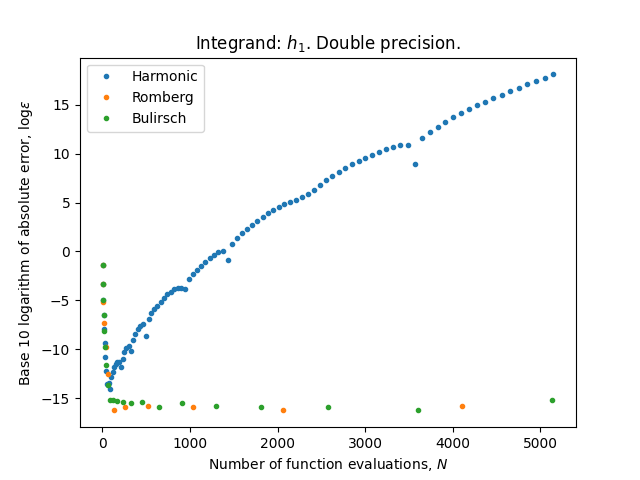
\includegraphics[scale=0.45]{romberg_plots/h_one.png}
\end{minipage}
\begin{minipage}{0.45\textwidth}
\centering
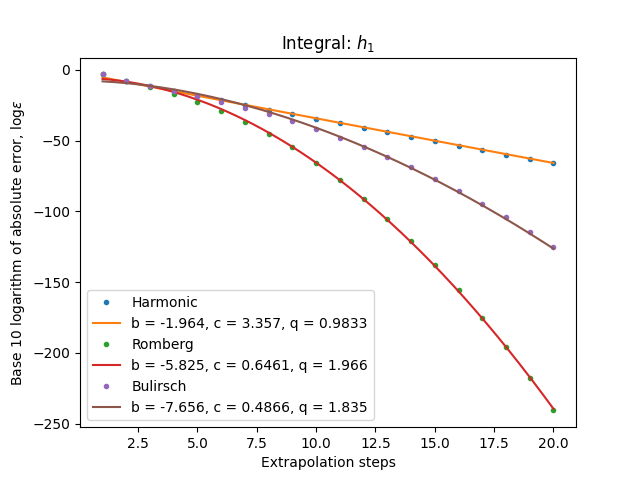
\includegraphics[scale=0.45]{romberg_plots/h_one_hp_steps.png}
\end{minipage}
\end{figure}

\begin{figure}[H]
\centering
\begin{minipage}{0.45\textwidth}
\centering
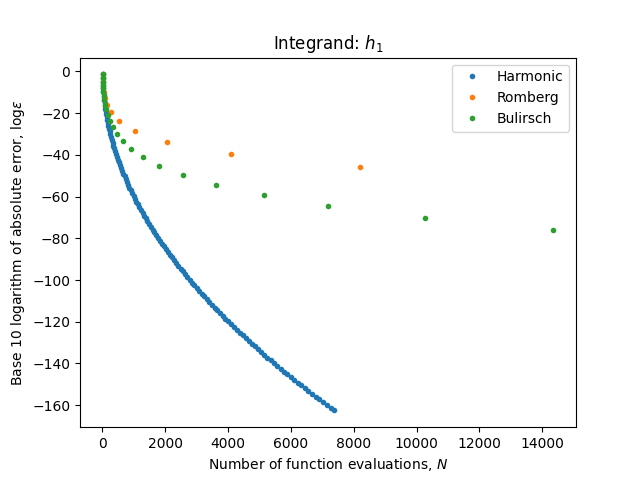
\includegraphics[scale=0.45]{romberg_plots/h_one_hp.png}
\end{minipage}
\begin{minipage}{0.45\textwidth}
\centering
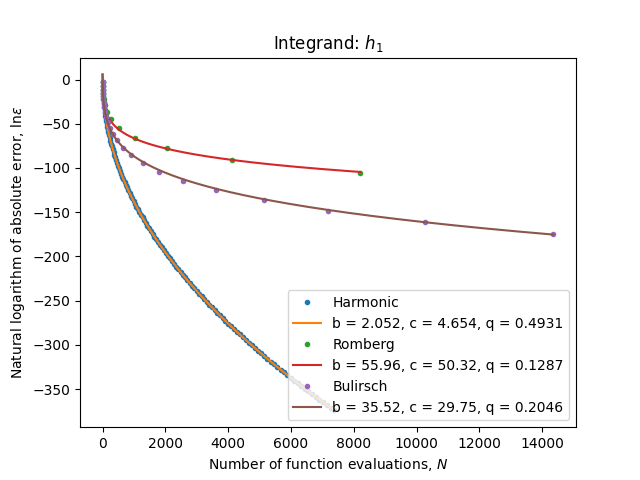
\includegraphics[scale=0.45]{romberg_plots/h_one_hp_trend.png}
\end{minipage}
\end{figure}

For \(a = 1\) the error seems to converge exponentially with the number of extrapolation steps for the harmonic sequence but the \(b\) parameters are suspicuously large for the other sequences. The error seems to converge exponentially with the number of extrapolation steps. The harmonic sequence results in the fastest convergence in the long run, then Bulirsch and then Romberg. In standard floating point arithmetic, we get down to machine level precision using Romberg and Bulirsch but not by using the Harmonic sequence.

\begin{figure}[H]
\centering
\begin{minipage}{0.45\textwidth}
\centering
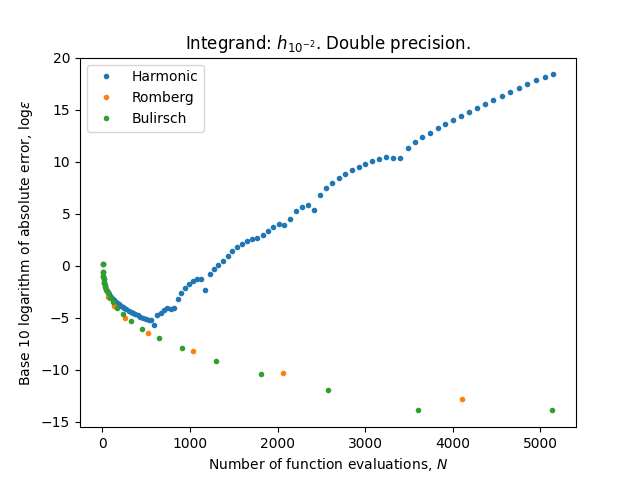
\includegraphics[scale=0.45]{romberg_plots/h_hundredth.png}
\end{minipage}
\begin{minipage}{0.45\textwidth}
\centering
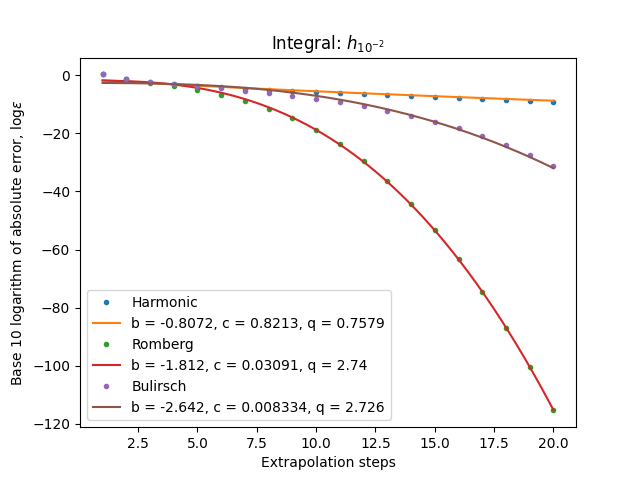
\includegraphics[scale=0.45]{romberg_plots/h_hundredth_hp_steps.png}
\end{minipage}
\end{figure}

\begin{figure}[H]
\centering
\begin{minipage}{0.45\textwidth}
\centering
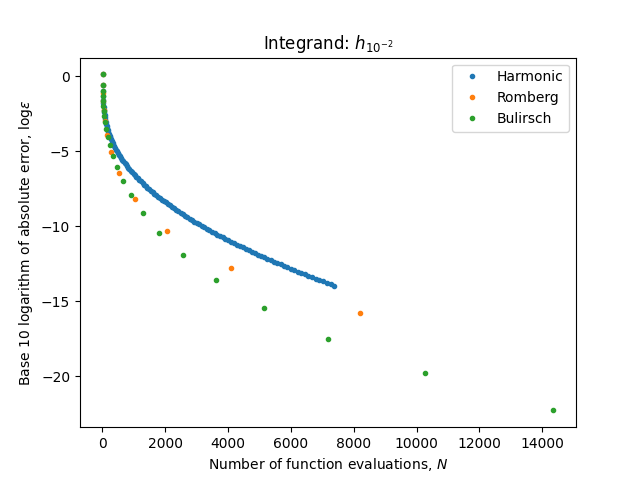
\includegraphics[scale=0.45]{romberg_plots/h_hundredth_hp.png}
\end{minipage}
\begin{minipage}{0.45\textwidth}
\centering
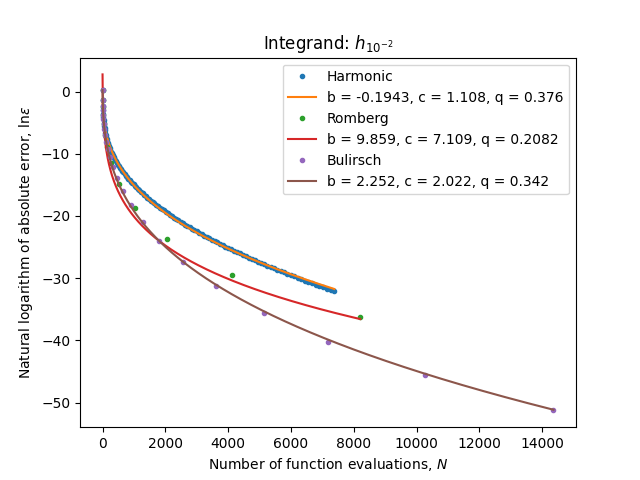
\includegraphics[scale=0.45]{romberg_plots/h_hundredth_hp_trend.png}
\end{minipage}
\end{figure}

\begin{figure}[H]
\centering
\begin{minipage}{0.45\textwidth}
\centering
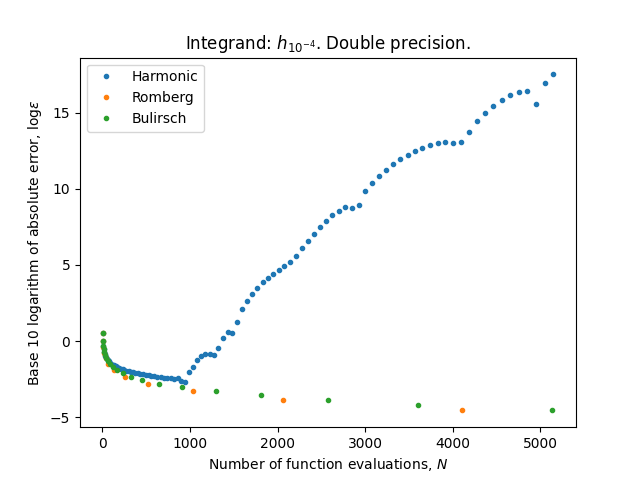
\includegraphics[scale=0.45]{romberg_plots/h_tenthousandth.png}
\end{minipage}
\begin{minipage}{0.45\textwidth}
\centering
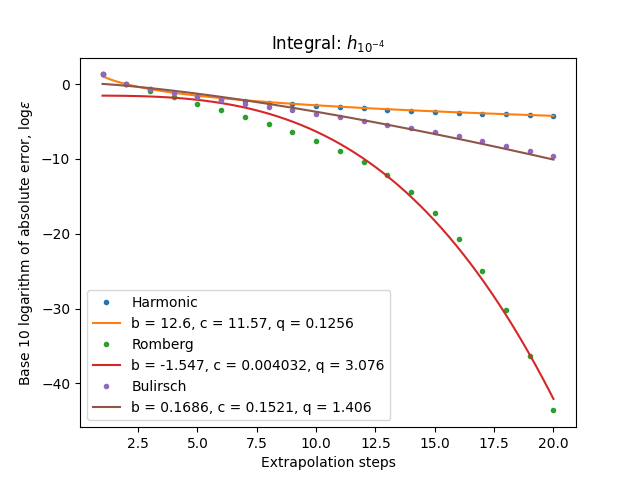
\includegraphics[scale=0.45]{romberg_plots/h_tenthousandth_hp_steps.png}
\end{minipage}
\end{figure}

\begin{figure}[H]
\centering
\begin{minipage}{0.45\textwidth}
\centering
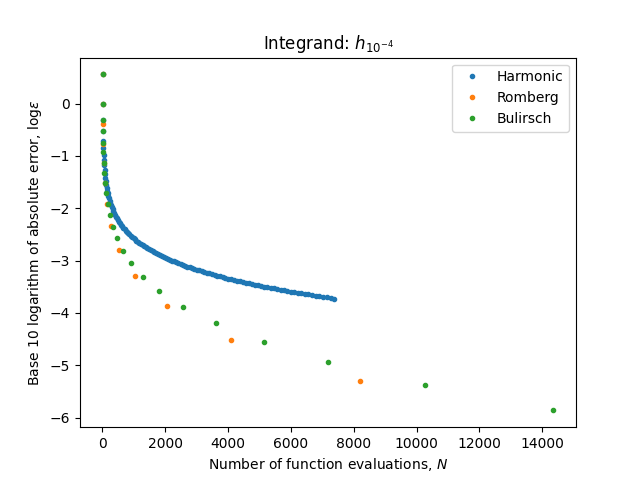
\includegraphics[scale=0.45]{romberg_plots/h_tenthousandth_hp.png}
\end{minipage}
\begin{minipage}{0.45\textwidth}
\centering
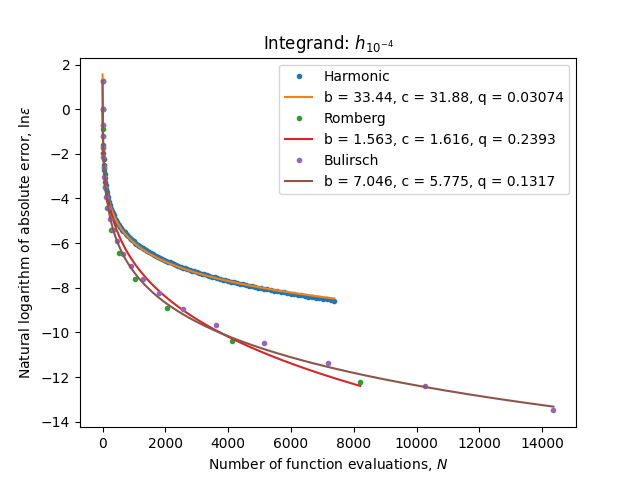
\includegraphics[scale=0.45]{romberg_plots/h_tenthousandth_hp_trend.png}
\end{minipage}
\end{figure}

For \(a = 10^{-2},\, 10^{-4}\) the parameters in the fitting of the number of function evaluations against the error seem more reasonable then the ones the fitting of the number of extrapolation steps against the error. The harmonic sequence performes not as well as the other two and in standard floating point precision we do not get down to the same level of accurracy using that.\\

If we plot the value of the optimal parameter \(q\) against \(a\), the resulting graph looks as follows: 

\begin{figure}[H]
\centering
\begin{minipage}{0.45\textwidth}
\centering
\includegraphics[scale=0.45]{romberg_plots/log_p_vs_q_h_a_by_param.png}
\end{minipage}
\end{figure}

\subsection{Area of half circle}

Now we will try the following function:
\[
i: [-1, 1] \rightarrow \R, \quad i(x)\coloneqq \sqrt{1-x^2}.
\]
This function is analytic inside the interval of definition but not at the endpoints. Its derivative has singularities at the endpoints.

\begin{figure}[H]
\centering
\begin{minipage}{0.45\textwidth}
\centering
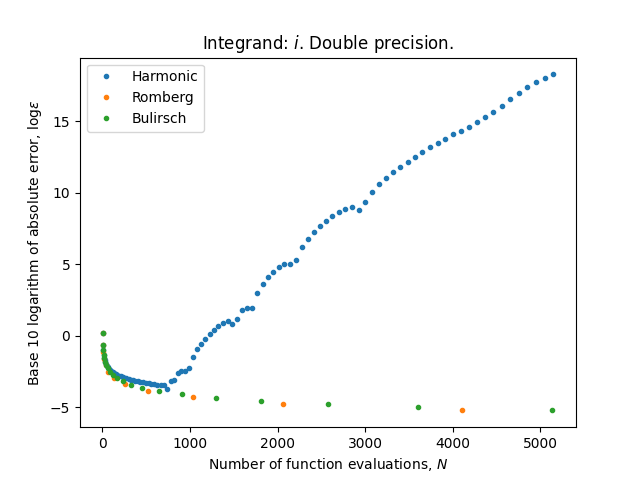
\includegraphics[scale=0.45]{romberg_plots/circle_area.png}
\end{minipage}
\begin{minipage}{0.45\textwidth}
\centering
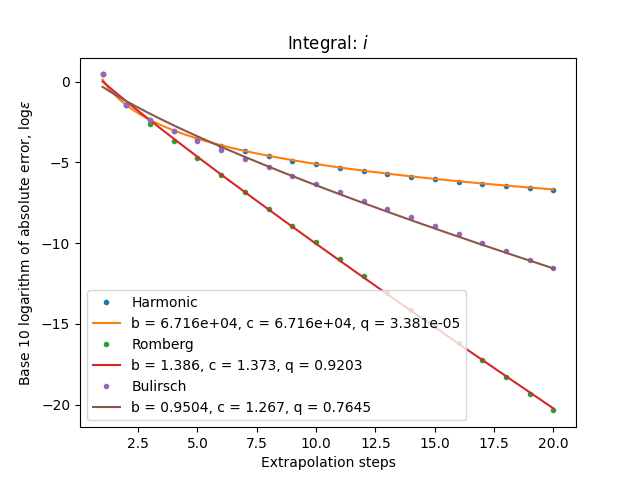
\includegraphics[scale=0.45]{romberg_plots/circle_area_hp_steps.png}
\end{minipage}
\end{figure}

\begin{figure}[H]
\centering
\begin{minipage}{0.45\textwidth}
\centering
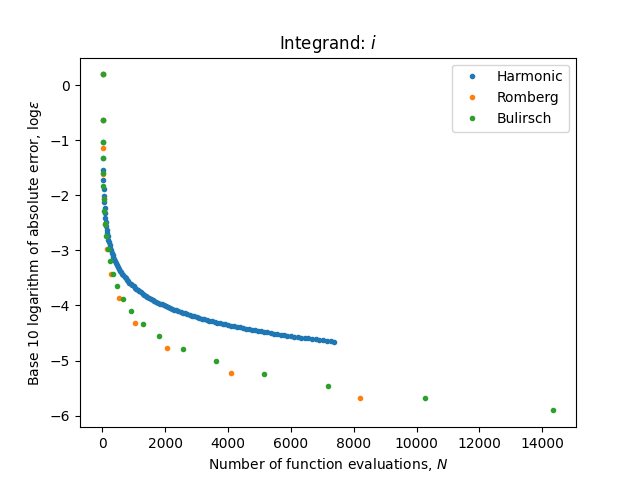
\includegraphics[scale=0.45]{romberg_plots/circle_area_hp.png}
\end{minipage}
\begin{minipage}{0.45\textwidth}
\centering
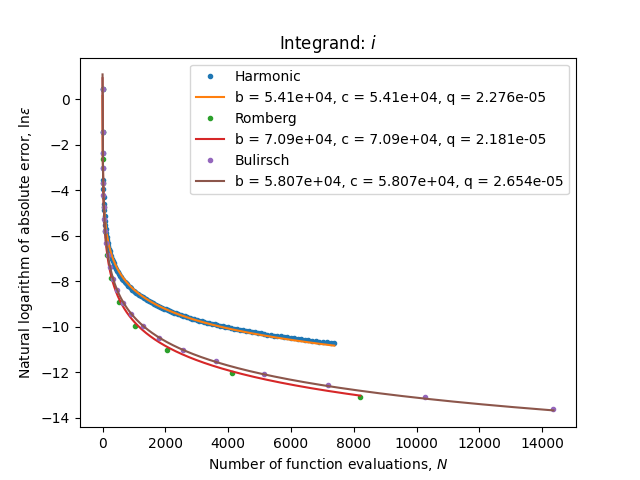
\includegraphics[scale=0.45]{romberg_plots/circle_area_hp_trend.png}
\end{minipage}
\end{figure}

Here the fit seems to be very unstable since we are getting very small values \(q\). Thus we shall try to plot a log-log plot of the number of evaluation agains the error. It looks as follows: 

\begin{figure}[H]
\centering
\begin{minipage}{0.45\textwidth}
\centering
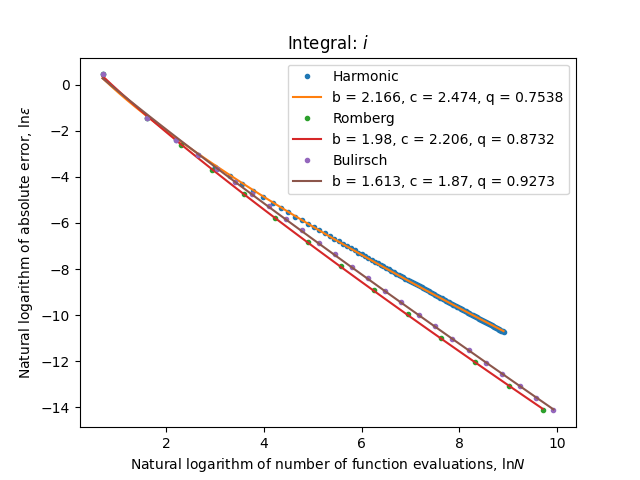
\includegraphics[scale=0.45]{romberg_plots/circle_area_hp_log_log_pow_fit_trend.png}
\end{minipage}
\end{figure}

We see that the values seem to fit on a line. Thus the relation seems to be rather \(\ln \varepsilon_i \sim a\ln N_i + b \) i.e. \(\varepsilon_i \sim C N_i^a\) which we call algebraic convergence.\\

\subsection{Gaussian}

Finally we will consider the Gaussian function
\[
j: [0,1]\rightarrow \R, \quad k(x) \coloneqq \frac{2}{\sqrt{\pi}} e^{-x^2}.
\]
\begin{figure}[H]
\centering
\begin{minipage}{0.45\textwidth}
\centering
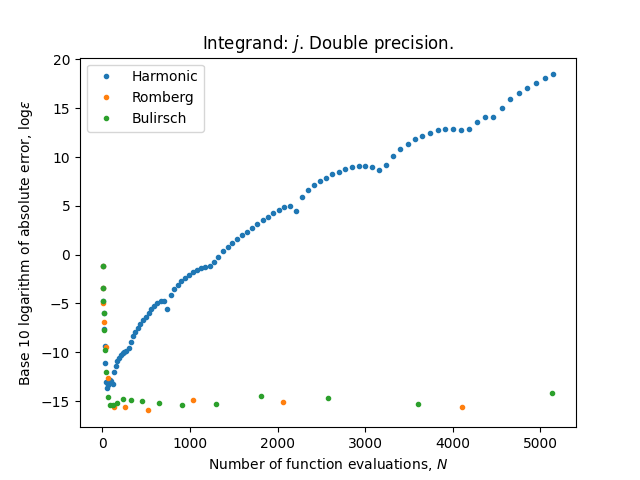
\includegraphics[scale=0.45]{romberg_plots/gaussian.png}
\end{minipage}
\begin{minipage}{0.45\textwidth}
\centering
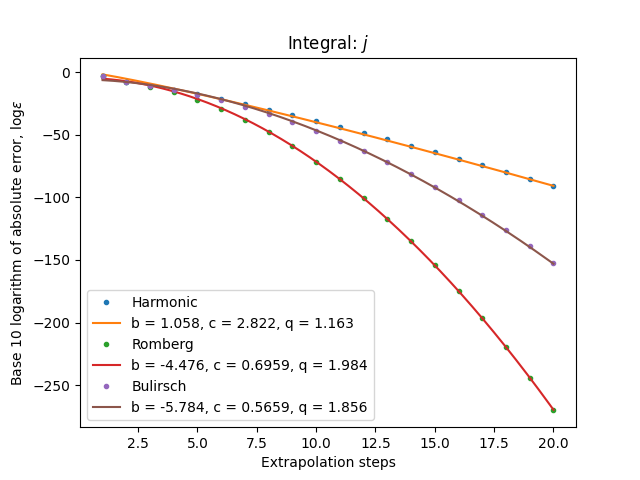
\includegraphics[scale=0.45]{romberg_plots/gaussian_hp_steps.png}
\end{minipage}
\end{figure}

\begin{figure}[H]
\centering
\begin{minipage}{0.45\textwidth}
\centering
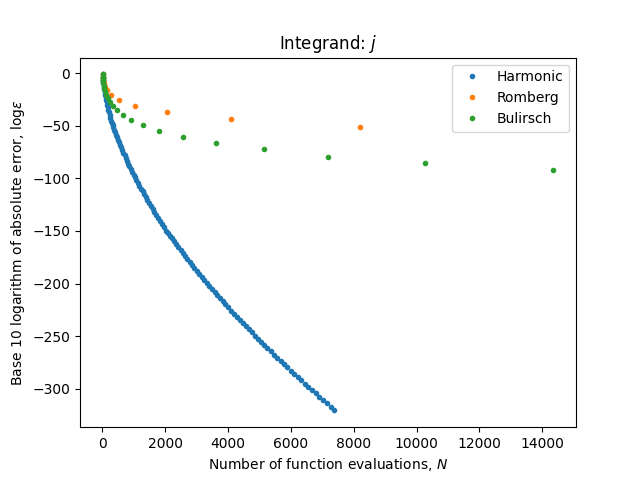
\includegraphics[scale=0.45]{romberg_plots/gaussian_hp.png}
\end{minipage}
\begin{minipage}{0.45\textwidth}
\centering
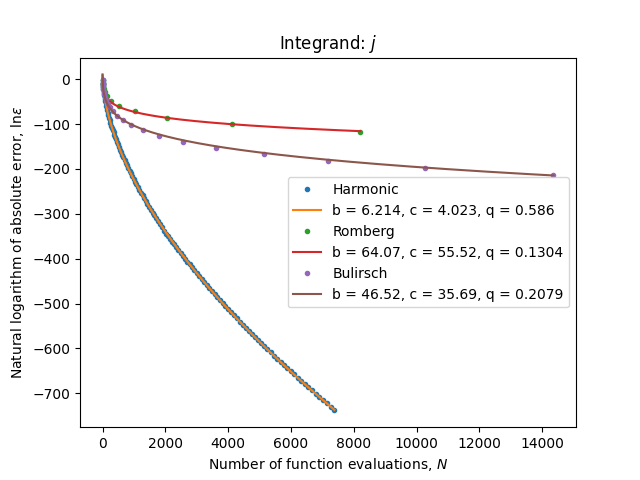
\includegraphics[scale=0.45]{romberg_plots/gaussian_hp_trend.png}
\end{minipage}
\end{figure}

Here the error seems to converge exponentially with the number of function evaluations for the harmonic sequence. For the other sequences the \(b\) parameters are unreasonably large. The error seems to converge exponentially with the number of extrapolation steps, in all cases. The harmonic sequence performes best, then Bulirsch an then Romberg. Using standard double precision, we get almost down to machine level precision using Romberg or Bulirsch, but are approximately \(2\) digits from there, using the Harmonic sequence.

The values of the optimal parameters in the curve fitting of evaluations against the logarithm of the error are:

\begin{table}[H]
    \centering
    \begin{tabular}{c|c||c|c|c}
        Integrand & Sequence & \(b\) & \(c\) & \(q\) \\\hline\hline
$f$ & Harmonic & \(15.66\) & \(3.1537\) & \(0.63887\) \\
$f$ & Romberg & \(30.844\) & \(22.442\) & \(0.2014\) \\
$f$ & Bulirsch & \(46.309\) & \(29.549\) & \(0.22556\) \\
$g_{10^{-2}}$ & Harmonic & \(5.7088\) & \(-0.8668\) & \(0.52546\) \\
$g_{10^{-2}}$ & Romberg & \(9.3083\) & \(0.96199\) & \(0.35893\) \\
$g_{10^{-2}}$ & Bulirsch & \(9.1445\) & \(0.49433\) & \(0.43743\) \\
$g_{10^{-1}}$ & Harmonic & \(2.2352\) & \(-0.66129\) & \(0.51817\) \\
$g_{10^{-1}}$ & Romberg & \(9.3824\) & \(3.6029\) & \(0.29851\) \\
$g_{10^{-1}}$ & Bulirsch & \(10.844\) & \(2.8849\) & \(0.34731\) \\
$g_1$ & Harmonic & \(1.6178\) & \(1.823\) & \(0.49467\) \\
$g_1$ & Romberg & \(23.192\) & \(18.171\) & \(0.19817\) \\
$g_1$ & Bulirsch & \(24.613\) & \(15.795\) & \(0.24492\) \\
$h_{10^{-4}}$ & Harmonic & \(33.436\) & \(31.879\) & \(0.030738\) \\
$h_{10^{-4}}$ & Romberg & \(9.6285\) & \(8.0889\) & \(0.1106\) \\
$h_{10^{-4}}$ & Bulirsch & \(7.0462\) & \(5.7755\) & \(0.13169\) \\
$h_{10^{-2}}$ & Harmonic & \(-0.19426\) & \(1.1078\) & \(0.37602\) \\
$h_{10^{-2}}$ & Romberg & \(4.3792\) & \(3.631\) & \(0.26761\) \\
$h_{10^{-2}}$ & Bulirsch & \(2.2519\) & \(2.0217\) & \(0.34203\) \\
$h_1$ & Harmonic & \(2.052\) & \(4.6543\) & \(0.4931\) \\
$h_1$ & Romberg & \(33.542\) & \(31.468\) & \(0.16462\) \\
$h_1$ & Bulirsch & \(35.525\) & \(29.752\) & \(0.20461\) \\
$i$ & Harmonic & \(54099\) & \(54099\) & \(2.2756\cdot 10^{-5}\) \\
$i$ & Romberg & \(55368\) & \(55367\) & \(2.8621\cdot 10^{-5}\) \\
$i$ & Bulirsch & \(58074\) & \(58073\) & \(2.6538\cdot 10^{-5}\) \\
$j$ & Harmonic & \(6.2138\) & \(4.0228\) & \(0.58595\) \\
$j$ & Romberg & \(33.68\) & \(30.265\) & \(0.17797\) \\
$j$ & Bulirsch & \(46.521\) & \(35.69\) & \(0.20788\) \\
    \end{tabular}
    \caption{Optimal parameters by test case}
    \label{tab:my_label}
\end{table}

The values of the optimal parameters in the curve fitting of extrapolation steps against the logarithm of the error are:

\begin{table}[H]
    \centering
    \begin{tabular}{c|c||c|c|c}
        Integrand & Sequence & \(b\) & \(c\) & \(q\) \\\hline\hline
$f$ & Harmonic & \(10.466\) & \(2.1696\) & \(1.2654\) \\
$f$ & Romberg & \(1.5206\) & \(0.51255\) & \(2.089\) \\
$f$ & Bulirsch & \(0.77673\) & \(0.41734\) & \(1.9549\) \\
$g_{10^{-2}}$ & Harmonic & \(6.5675\) & \(-0.61916\) & \(1.0458\) \\
$g_{10^{-2}}$ & Romberg & \(7.3378\) & \(0.0066103\) & \(3.1744\) \\
$g_{10^{-2}}$ & Bulirsch & \(7.3047\) & \(0.00063882\) & \(3.3913\) \\
$g_{10^{-1}}$ & Harmonic & \(2.8699\) & \(-0.47343\) & \(1.0317\) \\
$g_{10^{-1}}$ & Romberg & \(3.1888\) & \(0.039167\) & \(2.7667\) \\
$g_{10^{-1}}$ & Bulirsch & \(3.9142\) & \(0.012441\) & \(2.7293\) \\
$g_1$ & Harmonic & \(0.034332\) & \(1.3144\) & \(0.98632\) \\
$g_1$ & Romberg & \(-0.4289\) & \(0.41763\) & \(2.0726\) \\
$g_1$ & Bulirsch & \(-1.3077\) & \(0.18952\) & \(2.0725\) \\
$h_{10^{-4}}$ & Harmonic & \(12.604\) & \(11.571\) & \(0.12559\) \\
$h_{10^{-4}}$ & Romberg & \(0.85129\) & \(0.27953\) & \(1.4991\) \\
$h_{10^{-4}}$ & Bulirsch & \(0.16861\) & \(0.15206\) & \(1.4061\) \\
$h_{10^{-2}}$ & Harmonic & \(-0.80722\) & \(0.82135\) & \(0.75792\) \\
$h_{10^{-2}}$ & Romberg & \(-1.309\) & \(0.051824\) & \(2.5402\) \\
$h_{10^{-2}}$ & Bulirsch & \(-2.6424\) & \(0.0083341\) & \(2.7259\) \\
$h_1$ & Harmonic & \(-1.9642\) & \(3.3575\) & \(0.98328\) \\
$h_1$ & Romberg & \(-4.397\) & \(0.86863\) & \(1.8535\) \\
$h_1$ & Bulirsch & \(-7.6558\) & \(0.48664\) & \(1.8348\) \\
$i$ & Harmonic & \(67160\) & \(67160\) & \(3.3808\cdot 10^{-5}\) \\
$i$ & Romberg & \(1.8004\) & \(1.6494\) & \(0.85593\) \\
$i$ & Bulirsch & \(0.95043\) & \(1.2669\) & \(0.7645\) \\
$j$ & Harmonic & \(1.0579\) & \(2.8215\) & \(1.1626\) \\
$j$ & Romberg & \(-3.906\) & \(0.77717\) & \(1.9416\) \\
$j$ & Bulirsch & \(-5.7837\) & \(0.56594\) & \(1.8564\)
    \end{tabular}
    \caption{Optimal parameters by test case}
    \label{tab:my_label}
\end{table}